\chapter{Arithmetic of Fully Homomorphic Encryption Algorithm}
\label{Chapter3}
\section{An Efficient Fully Homomorphic Encryption Scheme} \label{3.1}
The proposed fully homomorphic encryption as in section \ref{FHE} is computationally inefficient because it executes a number of refresh or recrypt operations, over the encrypted data. At run-time, the time taken to perform a computation on cloud should not be more than the time taken by user to perform the entire computation by himself. The implementation supported in [\ref{fhew1}] provides a new technique to improve the efficiency of the proposed FHE implementation given in [\ref{lattices}].

The current implementation is used for computing the NAND of two encrypted bits, where the initial encryption is an learning with errors (LWE) based encryption. LWE encryption provides additive homomorphism. If a modulo 2 operation is used, it is possible to compute XOR of two numbers, homomorphically. However the technique given in [\ref{fhew1}] uses modulo 4 operation such that it results in computation of logical NAND. The bootstrapping method used in this technique is a ring variant, which efficiently computes modulo q operation over scalars. Other than this, ring variants allow the use of FFT techniques which help in reduction of computation time.
\subsection{Rounding Function}\label{roundingf}
    A rounding  function is defined  for integer n, such that 
    
    \hspace{3cm} $Rounding(X+n)=Rounding(X)+n$.
    
    \noindent In this distribution, $(Rounding(x)-x)$ is called the rounding error. If the domain of rounding function in restricted it adds a fixed noise to the input. 

\subsection{LWE Encryption}
\begin{itemize}
\item
\textbf{LWE Parameters:} \label{param}The various parameters used for LWE encryption are:
\begin{enumerate}
\item
Dimension: It is denoted by n. It denotes the dimension of the polynomials.
\item
Message Modulus: It is denoted by t. For the given scheme it is usually greater than or equal to 2. It is a factor by which the message is divided such that the noise is reduced. 
\item
Ciphertext Modulus: It is denoted by q. It is a factor with which the overall ciphertext is divided to reduce the noise and add semantic security.
\item
Rounding Function: As referenced in section \ref{roundingf}, a rounding function adds noise to the input. In the given technique the rounding function works in a way such that the introduced noise is always less than $(q/(2\times t))$.
\end{enumerate}
\item
\textbf{LWE Encryption:} Given a message m and a secret key s, the LWE encryption of m under the secret key s, is given as

\hspace{3cm}
$LWE\textsubscript{s}(m)=Rounding(a\times s+((m\times q)/t))\bmod q$,

where a is chosen at random and t \& q are the LWE parameters as defined in section \ref{param}.
\item
\textbf{LWE Decryption:} Given a ciphertext b and a secret key s, the LWE decryption of b to get m, under the secret key s, is given as

\hspace{3cm}
  $m=\lfloor{t\times (b-a\times s)/q}\rfloor \bmod t$  


where a is chosen at random and t \& q are the LWE parameters as defined in section \ref{param}.
\item
\textbf{Rounding Error:} The rounding error of a ciphertext is given as: 

\hspace{3cm}$error=(b-a\times s-mq/t)\bmod q$,

which is the reduced error by modulo q, so that it lies within the interval $[-q/2, q/2]$.
\item
\textbf{Modulus Switching:} At times a ciphertext in one form with a modulus q can be converted to another ciphertext, which has a different modulus $q^{'}$, by a process called switching of modulus. Given b as a LWE cipher text with modulus q, then $b^{'}$ with modulus $q^{'}$, can be derived from b by the following expression:

\hspace{3cm}$b^{'}=\lfloor{(q^{'}\times b)/q}\rfloor +B$

where B is a random variable with value ranging between 0 to 1.
\item
\textbf{Key Switching:} It is a procedure under which an encryption of a message under a key pk\textsubscript{1} results in another encryption of the same message under a different key. 
\end{itemize}
\subsection{Logical NAND using FHE} \label{3.1.2}
Given two LWE ciphertexts c\textsubscript{1} and c\textsubscript{2} which are the encryptions of m\textsubscript{1} and m\textsubscript{2} encrypted with message modulus $t=2$ and ciphertext modulus q. The aim is to compute a logical NAND operation homomorphically such that the resultant is an LWE encryption of NAND of m\textsubscript{1} and m\textsubscript{2} with message modulus $t=2$ and cipher text modulus q. The implementation as proposed in [\ref{fhew1}] achieves this with the help of following steps.

\begin{itemize}
\item
\textbf{HOMNAND:} It is an algorithm wherein message modulus $t=4$, and error range between $-q/16$ to $q/16$ is used for the initial encryption of two input bits m\textsubscript{1} and  m\textsubscript{2}. The multiplication of these two encrypted bits result in a LWE ciphertext which is an encryption of result of logical NAND on m\textsubscript{1} and  m\textsubscript{2} with an error bound of $q/4$.
i.e.

$LWE\textsubscript{s}(m\textsubscript{1},q/16)\times LWE\textsubscript{s}(m\textsubscript{2},q/16)$ results in $LWE\textsubscript{s}(m\textsubscript{1}$NAND $m\textsubscript{2},q/4)$

\vspace{0.25cm}
\noindent HOMNAND algorithm computes the NAND of two ciphertexts by using addition but the noise increases up to a maximum value of $q/4$ and this noise or error needs to be limited i.e. a refresh operation needs to be performed such that the resultant ciphertext has a noise bound as $q/16$ and not $q/4$. It is also known that the number of refresh computations is bounded by the depth of the circuit and the number of inputs to each gate. The high cost of evaluation is limited by initially changing the message modulus and ciphertext modulus such that already a recrypted input is supplied to the circuit, which limits the number of refresh computations. 
\item
\textbf{Refresh:} Refresh operation is performed with the help of homomorphic accumulator. It is performed with the help of two encryption algorithms, where in the first encryption is LWE encryption and the second encryption scheme is used by the accumulator internally to homomorphically evaluate the LWE decryption on the encrypted secret key.
Refresh procedure takes as input an LWE ciphertext with noise bound of $q/4$, which is the result of HOMNAND and a refreshing key. The refresh operation is performed by the homomorphic accumulator with the help of four operations.
\begin{enumerate}
\item
\textbf{Encryption:} It is an intermediate encryption scheme which is used to encrypt the secret key s, and allows the transformation $b-a\times Enc(s)$ which is a step for LWE decryption.
\item
\textbf{Initialize:} The accumulator is initialized to a value $b+q/4$, where b is the ciphertext and q is the ciphertext modulus. This operation sets up accumulator with a noiseless encryption of v under the above encryption scheme with a key s.
\item
\textbf{Increment:} The accumulator is incremented by adding a number of independent and freshly generated ciphertexts. An efficient algorithm for incrementing the accumulator is implemented by using FFT techniques.
\item
\textbf{MSB Extract:} The most significant bit of the accumulator is extracted, which is the final LWE encrypted result of the NAND computation with noise in the range. It uses \textit{Keyswitch} and \textit{Modswitch} algorithms of LWE in practice.
\end{enumerate}
\end{itemize}
%figure
\begin{figure}[!h]
\centering
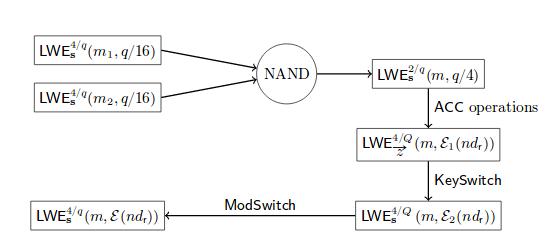
\includegraphics[scale=0.7]{figures/NAND.png}
\caption{Cycle of NAND Computation (Source[\ref{fhew1}])}
\label{fig:NAND cycle}
\end{figure}

\noindent The result after performing the refresh is an LWE encryption of the logical NAND operation performed on LWE encryption of two bit inputs, with the noise bounded in the range $q/16$. It should be noted that in the above figure, \textit{E(nd\textsubscript{r})} is $q/16$, to have the final noise bound in the resulting ciphertext as $q/16$. Refresh operation takes a lot of computation overhead in the implementation, which increases with the increase in number of gates or the depth of the circuit.


\section{Introduction to FHEW Library} \label{3.2}
The library referenced  in [\ref{fhewlib}] gives an open source working implementation of [\ref{fhew1}] in C++. It supports encryption and decryption of single bit messages, using LWE symmetric encryption scheme and also evaluation or homomorphic computation of boolean functions using the public encryption key. The main features of the library useful for the analysis of this report are referenced below:
\begin{itemize}
\item
FHEW::setup(): The library uses this function, to setup the dimensions and plan of FFT, and also to generate a test MSB. 
\item
Two random bits are generated and LWE encrypted, using the LWE secret key which is an integer array of dimension 500.
\item
FHEW::keyGen: This uses FHEW\_Encrypt() function and generates an evaluation key from the LWE secret key. Evaluation key is a packed structure variable holding the bootstrapping key and the switching key. It is generated with the help of forward and backward FFT operations. The dimensions of the bootstrapping key and switching key are 1032 MB and 314 MB respectively.
\item
FHEW::HomNAND(): It takes two LWE ciphertexts as input and performs HomNAND operation based on the method as given in the section \ref{3.1.2}. The product is computed with the usage of FFT in the library. It takes about 48000 FFT computations for a single HOMNAND operation.
\item
LWE::Keyswtich() and  LWE::ModSwitch(): Modswitch and Key switch functions are used to further reduce the noise in the ciphertext.
\item
FFT computation is executed with the usage of FFTW3 Library, which yields a fast software implementation of FFT.
\end{itemize}

\section{FFTW Library}
FFTW library allows to compute any arbitrary dimension FFT, for both real and complex data. The main features of the library used in the implementation of FHEW are described below:
\begin{enumerate}
\item
\textbf{fftw\_complex Datatype}: It is an array of 2 elements of double datatype, where the first index stores the real part and the second index stores the imaginary part of a complex number.
\item
\textbf{fftwf\_malloc Function:} This function behaves as malloc i.e. it allocates the transform data. The data is aligned in a manner such that a speedup is acquired if the data is accessed for multiple instructions single data execution.

\noindent Examples usages of fftwf\_malloc:
\begin{itemize}
\item
(double*)fftw\_malloc(sizeof(double)*N)
\item
(fftw\_complex*)fftw\_malloc(sizeof(fftw\_complex)*N)
\end{itemize}
Alternatively some wrappers are also provided corresponding to the above two examples e.g. fftw\_alloc\_real(N) for real data allocation and fftw\_alloc\_complex(N) for complex memory allocation, where N is the dimension of the data.
\item
\textbf{fftwf\_free Function:} This function is corresponding to the fftwf\_malloc function to deallocate the memory allocated to transform data.
\item
\textbf{fftw\_plan Datatype:} fftw\_plan is an object. It stores all the data necessary to compute an FFT operation. It also contains the details and pointers to input and output arrays. 
\item
\textbf{Creating a Plan:} There are several functions available to create FFT plans, which are stored in fftw\_plan object based on the dimensions of the FFT. e.g. 1D, 2D, 3D plans etc.
As examples the following functions are used to create plans for 1 Dimensional FFT's on real data. 
\begin{itemize}
\item
fftw\_plan fftw\_plan\_dft\_r2c\_1d(int n, double *in, fftw\_complex *out,unsigned flags);

This creates a plan for a one dimensional real input to the complex output (r2c) transform, which is usually the case for forward FFT.
\vspace{0.25cm}
\item
fftw\_plan fftw\_plan\_dft\_c2r\_1d(int n, fftw\_complex *in, double *out,unsigned flags);

This is creates a plan for a one dimensional complex input to real output (c2r) transform, which is usually the case for inverse FFT.
\end{itemize}
There are various flags available for the decision on plans e.g. 

- FFTW\_ESTIMATE picks up an optimal plan based on some heuristic.

- FFTW\_PATIENT generates an plan based on a wide range of algorithms but it takes a long time to pick up a plan.

- FFTW\_MEASURE is the default plan of the library. It picks up a plan based on the measurement of execution time of computation of several FFT's.

Other options available are FFTW\_EXHAUSTIVE and FFTW\_WISDOM\_ONLY, which are based on an even wider range of algorithms to pick up a plan. 
\item
\textbf{Executing a Plan:} After a plan is created it can be executed using the following function:

void fftw\_execute(const fftw\_plan plan)

A plan can be executed any number of times, by providing the input and output variables.
\item
\textbf{Deallocating a Plan:} A plan can be deallocated using the function:

void fftw\_destroy\_plan(fftw\_plan plan)

 \end{enumerate}
 The library can be installed for single precision float, double precision float, long double and also for quad precision. The above functions can be modified to support the corresponding functions for the desired precision. To modify, the corresponding function names should be updated by replacing the ‘fftw\_’ with ‘fftwf\_’ for single precision floating point, or ‘fftwl\_’ for long double and so on.
 
 \noindent The corresponding linking libraries are also changed e.g. for quadratic precision, the linker libraries are changed from -lfftw3 to -lfftw3q. Also the math libraries are needed to be linked for quadratic precision i.e. -lquadmath -lm. 
 \section{Setting up FHEW}
\begin{itemize}
\item
FHEW library can be cloned from the git repository \textit{"Implementation of FHEW, by L. Ducas and D. Micciancio"}[\ref{fhewlib}]. As this library uses \textit{"Fast fourier Transform in the west (FFTW)"} library for faster computation of fast fourier transform to execute the homomorphic accumulator, FFTW needs to be setup as a prerequisite to setting up FHEW.
\subsection{Setting up FFTW} \label{3.4.1}
\begin{itemize}
\item
FFTW can be downloaded as a tar file in linux operating system from [\ref{fftw}]. Alternatively it can also be cloned from the git repository as referred in [\ref{FFTW3git}], but this requires additional steps such as installation of certain tools, to automatically generate the source code.
\item
The file needs to be untar to extract the library files and the current directory is set to the library folder for further steps.
\item 
A C compiler is needed to execute and build the fftw files. Before building the library the \textit{makefile} needs to be configured using the configure program which is executed using the command

\hspace{3cm} ./configure

\item
After the \textit{makefile} is configured, the library can be built and installed using \textit{make} and \textit{make install} commands. The library is installed for double precision FFT operations by default.
\end{itemize}
\item
After FFTW is setup, FHEW can be built using the command \textit{make} by setting the FHEW library folder as the present working directory. After running the make, a library folder \textit{Libfhew.a} is created in the working directory.
\item
The command \textit{"make install"} helps the user to install the header files necessary to run user defined programs or test applications provided.
\item
The library can be tested by running the test program \textit{fhewtest}, which takes as an argument the number of NAND operations to be performed in one iteration or in other words the depth of the circuit.
The library can be tested for e.g. one NAND gate computation as:

\hspace{3cm}
./fhewtest 1
\item
If the test program is run without any arguments, a message is displayed, which tells about the correct execution of the library test code. Running the command with argument as alphabet "n", tests the application with a circuit depth of 0, that is performs no NAND operation. e.g.

\hspace{3cm}
./fhewtest n

tests the homomorphic NAND operation 0 times.
\end{itemize}
\section{FFT as Computationally Intense Algorithm of Library}
From the background information given in chapter[\ref{Chapter2}], we see the most computationally intense part of any fully homomorphic encryption scheme is the bootstrapping operation, which involves an evaluation of decryption function homomorphically, so as to reduce the noise in the final ciphertext. Bootstrapping is alternatively called refresh or recrypt operation because it gives the encryption of the result with a different public key, which offers lesser noise. Also the computational demand of the algorithm increases with the depth of operation which directly influences the number of refresh computations performed. The scheme described in section {\ref{3.1}}, gives an efficient method to perform bootstrapping using homomorphic accumulator algorithm for a logical NAND operation on two single bit data. 

The implementation of the scheme given in section {\ref{3.1}} executes the homomorphic accumulation algorithm with the help of fast fourier transforms, which are executed efficiently with the help of FFTW library. As per the benchmarking provided by the above implementation, there are about 48000 FFT's running for one Logical NAND computation. On thorough analysis of the code flow, it is devised that the most computationally intense function in the algorithm i.e. HOMNAND uses a significant amount of forward and backward double precision complex FFT's of a large dimension i.e. 2048. Other than this the function \textit{"FHEWencrypt"} for generation of bootstrapping key also performs encryption of secret key by running the FFT algorithm at the back end and consumes a significant amount of processing power.

Hence for further analysis of the module, FFT is chosen as the most computationally intense algorithm of the application because of its dimension and complexity.
\section{Rationale Behind Conversion from Double Precision to Single Precision Floating Point FFT}
Double precision floating point uses 64 bits to store a number wherein the first bit is the sign bit, the next 11 bits are used to store the exponent and the remaining bits are used as fraction as shown in figure \ref{fig:doublep} 

\begin{figure}[!h]
\centering
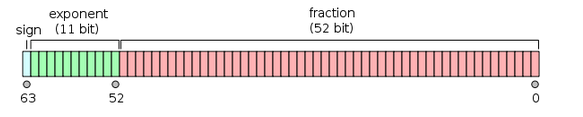
\includegraphics[scale=0.75]{figures/doublePrecison.png}
\caption{Double Precision Datatype Representation (Source [\ref{dp}])}
\label{fig:doublep}
\end{figure}
\noindent whereas single precision floating point uses 32 bits to store a number wherein the first bit is the sign bit, the next 8 bits are used to store the exponent and the remaining bits are used as fraction (Refer figure \ref{fig:Float Representation}). The extra bits in double precision allows to increase the precision and the range of numbers to be stored in a datatype. 

\noindent The FHEW library as described in section {\ref{3.2}} uses a 2048(power of 2) point FFT, because the reductions by modulo 2 are offered implicitly, however only the values at odd indexes of the result are used for further computations. As per the library, small errors introduced with the floating point approximations, can be neglected as the rounding errors. Also the results of the FFT's are directly rounded off to integers, instead FFT's are used to facilitate multiplication of two integer polynomials. 

\noindent The idea is to implement FHEW on hardware and hence conversion of the FFT to single precision float rather than double precision float, will consume significantly lesser number of resources for the computation. At the same time, it affects the speed of operation on the hardware by hence increasing the achievable parallelism. The input and output values of the FFT iterations were printed in respective files, with the help of modifications in code flow. The data was carefully studied are analyzed for the minimum and maximum values to validate the range of numbers (Refer table \ref{Table 3.1}).

\begin{table}[!h]
\centering
\caption{Range of Forward and Backward FFT output}
\label{Table 3.1}
\begin{tabular}{||m{4.5cm}|m{4.5cm}|m{4cm}||}
\hline
Metric & Minimum &Maximum\\[1.5ex]
\hline
\hline
\multirow{3}{*}{FFT Forward Output} & \multicolumn{2}{|c||}{Real Part}\\[1.5ex]
\cline{2-3}
 &-162956607488.0000000 &  160433176576.0000000  \\[1.5ex]
\cline{2-3}
 & \multicolumn{2}{|c||}{Imaginary Part} \\[1.5ex]
\cline{2-3}
 & -758385934336.0000000 &152867258368.0000000\\[1.5ex]
\hline
\hline
FFT Backward Output & -2147483579.0000000 & 2147483646.0000000\\[1.5ex]
\hline
\end{tabular}
\end{table}


If the values are analyzed for the range, as in table \ref{Table 3.1} it can be seen that the values can be accommodated in single precision floating point variable. Hence the conversion from double precision floating point to single precision floating point can be explored for optimization of resources on hardware. 
\section{Installing FFTW in both single and double precision}
By default FFTW is installed to support double precision floating point FFT. To modify FHEW for analysis of above assumption, it needs to be installed such that it supports single precision FFT.

Here the library is installed to support both double and single precision FFT computation, for it offers convenience to compare the results of single precision and double precision floating point for the same data. The reason for dual installation is that as the data used in encryption algorithms is randomly generated, so for effective analysis of results the data from both computations should be compared in the same iteration, as running the iteration separately will result in different data input.
\subsection{Steps for Setting up FFTW for both single and double precision}
\begin{itemize}
\item
If the library is already installed for double precision floating point, a clean build should be run. This can be done by running the command \textit{make clean} after setting the library folder as the working directory.
\item
The configure command as specified in section \ref{3.4.1} to configure the \textit{makefile} is modified to enable float. Hence the \textit{makefile} is configured to support both single and double precision FFT on the same system, by using the command

\hspace{3cm} ./configure --enable-float
\item
The library is rebuilt using \textit{make} and \textit{make install}  commands.
\end{itemize}
\section {Modifications to Code Flow}
The code flow for the FFT is modified to support the functions for single precision float.
\begin{itemize}
\item
The \textit{MakeFile} for FHEW is modified to link the fftw library with -lfftw3 and -lfftw3f where -lfftw3 supports library flag for double precision and -lfftw3f stores the library flags for single precision float.

\lstset { %
	language=C,
	backgroundcolor=\color{lightgray}, % set backgroundcolor
	%basicstyle=\footnotesize,% basic font setting
	basicstyle=\ttfamily\scriptsize,
	%\basicstyle=\ttfamily\scriptsize,
	keywordstyle=\color{blue}\ttfamily,
	stringstyle=\color{red}\ttfamily,
	commentstyle=\color{darkgray}\ttfamily,
	breaklines=true	
}
\lstset{framesep=-10pt, xleftmargin=-10pt}
\begin{lstlisting}[caption={FHEW: Makefile},label={listing:3.8.1}]
PREFIX=$(HOME)

CC=g++

AR=ar

CFLAGS= -ansi -Wall -O3

LDFLAGS= -L. -lfhew -lfftw3f -lfftw3

INCLUDE=distrib.h LWE.h FHEW.h FFT.h params.h

\end{lstlisting}




\item 
The data types or variables storing the double precision values are modified to float.
\lstset { %
	language=C,
	backgroundcolor=\color{lightgray}, % set backgroundcolor
	%basicstyle=\footnotesize,% basic font setting
	basicstyle=\ttfamily\scriptsize,
	%\basicstyle=\ttfamily\scriptsize,
	keywordstyle=\color{blue}\ttfamily,
	stringstyle=\color{red}\ttfamily,
	commentstyle=\color{darkgray}\ttfamily,
	breaklines=true	
}
\lstset{framesep=-10pt, xleftmargin=-10pt}
\begin{lstlisting}[caption={FHEW: FFT datatypes},label={listing:3.8.2}]
#include <fftw3.h>

// Parameters for FFT Computation in Single Precision Float

float *in_float;
fftwf_complex *out_float;
fftwf_plan plan_fft_forw_float, plan_fft_back_float;

// Parameters for FFT Computation in Double Precision Float

double *in_double;
fftw_complex *out_double;
fftw_plan plan_fft_forw_double, plan_fft_back_double;
\end{lstlisting}




\item
The various functions used for FFT are replaced with the corresponding functions for single precision floating point as shown in listing \ref{listing:3.8.3} to \ref{listing:3.8.5}.

\lstset { %
	language=C,
	backgroundcolor=\color{lightgray}, % set backgroundcolor
	%basicstyle=\footnotesize,% basic font setting
	basicstyle=\ttfamily\scriptsize,
	%\basicstyle=\ttfamily\scriptsize,
	keywordstyle=\color{blue}\ttfamily,
	stringstyle=\color{red}\ttfamily,
	commentstyle=\color{darkgray}\ttfamily,
	breaklines=true	
}
\lstset{framesep=-10pt, xleftmargin=-10pt}
\begin{lstlisting}[caption={FHEW: FFT Setup Function},label={listing:3.8.3}]
//FFT Setup function
void FFTsetup(){

//Sets up data to compute single precision float FFT

  in_float = (float*) fftwf_malloc(sizeof(float) * 2*N);
  out_float = (fftwf_complex*) fftwf_malloc(sizeof(fftwf_complex) * (N + 2));
  plan_fft_forw_float = fftwf_plan_dft_r2c_1d(2*N, in_float, out_float,  FFTW_PATIENT);
  plan_fft_back_float = fftwf_plan_dft_c2r_1d(2*N, out_float, in_float,  FFTW_PATIENT);

//Sets up data to compute single precision float FFT

  in_double = (double*) fftw_malloc(sizeof(double) * 2*N);
  out_double = (fftw_complex*) fftw_malloc(sizeof(fftw_complex) * (N + 2));
  plan_fft_forw_double = fftw_plan_dft_r2c_1d(2*N, in_double, out_double,  FFTW_PATIENT);
  plan_fft_back_double = fftw_plan_dft_c2r_1d(2*N, out_double, in_double,  FFTW_PATIENT);
}

\end{lstlisting}




\lstset { %
	language=C,
	backgroundcolor=\color{lightgray}, % set backgroundcolor
	%basicstyle=\footnotesize,% basic font setting
	basicstyle=\ttfamily\scriptsize,
	%\basicstyle=\ttfamily\scriptsize,
	keywordstyle=\color{blue}\ttfamily,
	stringstyle=\color{red}\ttfamily,
	commentstyle=\color{darkgray}\ttfamily,
	breaklines=true	
}
\lstset{framesep=-10pt, xleftmargin=-10pt}
\begin{lstlisting}[caption={FHEW: FFT Forward Function},label={listing:3.8.4}]
void FFTforward() {

//Executes Forward FFT for Single Precision Float
  fftwf_execute(plan_fft_forw_float); 
 
//Executes Forward FFT for Double Precision Float
  fftw_execute(plan_fft_forw_double); 
}

\end{lstlisting}




\lstset { %
	language=C,
	backgroundcolor=\color{lightgray}, % set backgroundcolor
	%basicstyle=\footnotesize,% basic font setting
	basicstyle=\ttfamily\scriptsize,
	%\basicstyle=\ttfamily\scriptsize,
	keywordstyle=\color{blue}\ttfamily,
	stringstyle=\color{red}\ttfamily,
	commentstyle=\color{darkgray}\ttfamily,
	breaklines=true	
}
\lstset{framesep=-10pt, xleftmargin=-10pt}
\begin{lstlisting}[caption={FHEW: FFT Backward Function},label={listing:3.8.5}]
void FFTbackward()
{

//Executes Inverse FFT for Single Precision Float
  fftwf_execute(plan_fft_back_float); 
 
//Executes Inverse FFT for Double Precision Float
  fftw_execute(plan_fft_back_double); 
}
\end{lstlisting}





\item
The datatype for other variables to hold the value for Test MSB, the bootstrapping Keys, switching keys which are generated as a result of FFT operations is changed to fftwf\_complex. 
\lstset { %
	language=C,
	backgroundcolor=\color{lightgray}, % set backgroundcolor
	%basicstyle=\footnotesize,% basic font setting
	basicstyle=\ttfamily\scriptsize,
	%\basicstyle=\ttfamily\scriptsize,
	keywordstyle=\color{blue}\ttfamily,
	stringstyle=\color{red}\ttfamily,
	commentstyle=\color{darkgray}\ttfamily,
	breaklines=true	
}
\lstset{framesep=-10pt, xleftmargin=-10pt}
\begin{lstlisting}[caption={FHEW Parameters},label={listing:3.8.6}]

\\This datatype is used to store Test MSB, Bootstrapping and Switching key Variables.
typedef fftwf_complex Ring_FFT[N2];

\end{lstlisting}





\end{itemize}
\section {Output for the Single Precision Float Modification}
The necessary code changes are made in the \textit{"FHEW.cpp"} file and it is executed for one execution of NAND gate. The single precision floating point was not supported by the library and the modification gives error in the computation as given in the figure \ref{fig:SPresults}.
%figure

\begin{figure}[!h]
\centering
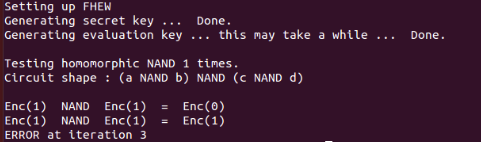
\includegraphics[scale=0.65]{figures/spresults.png}
\caption{Results of Single Precision Floating Point Modification}
\label{fig:SPresults}
\end{figure}
\section{ Analysis of results}\label{3.10}
This section presents the analysis of the results obtained after modifying the library for single precision float which in turn is not supported and generates an error. The possible causes of error as identified are:
\begin{itemize}
\item
\textbf{Error in FFT Computation:} From conceptual background, it is known that FFT is an algorithm to efficiently compute DFT, by limiting the number of operations. As per the results of [\ref{FFT accuracy}] FFT is as accurate as DFT, but still it is sensitive to the value of twiddle factors associated with the computation. Based on the paper [\ref{FFT accuracy}], the major sources of error associated in the computation are the following :
\begin{itemize}
\item
Computational errors in computing the FFT.
\item
Instability of DSP blocks used for computing FFT.
\item
Errors in twiddle factors which are the basis of FFT computation.
\item
Roundoff errors in case the result is rounded to be stored in a smaller data type variable.
\end{itemize}
Ideally the accuracy of twiddle factors  or the sine and cosine tables affect the accuracy of the FFT.
The RMS error in the computation of FFT for accurate sine and cosine tables for a N point transform is given as:

\noindent For single precision 32-bit IEEE floating point: 

\hspace{3cm} 0.6$\epsilon$\textsubscript{32}$\sqrt{\log{2}{N}}$ \hfill eqn[3.1]

\noindent For double precision 64-bit IEEE floating point:

\hspace{3cm}0.6$\epsilon$\textsubscript{64}$\sqrt{log{2}{N}}$\hfill eqn[3.2]

\noindent where 
\begin{math}
\epsilon
\end{math}
\textsubscript{32}= 5.96*$10^{-8}$ and $\epsilon$\textsubscript{64}=1.11*$10^{-16}$.
\noindent It can be seen from the equations eqn[3.1] and eqn[3.2] that the error in FFT computation with the use of 64 bit double precision floating point is significantly less as compared to 32 bit single precision floating point. The variation of the error is almost by a factor of $10^{8}$. 

Analyzing the accuracy of FFTW library from the reference [\ref{fftw}], it can be seen for double precision real data 1D transform the relative RMS error is close to a power of $10^{-16}$ for a 2048 point FFT as given in figure \ref{fig:doublea}.

\begin{figure}[!h]
\centering
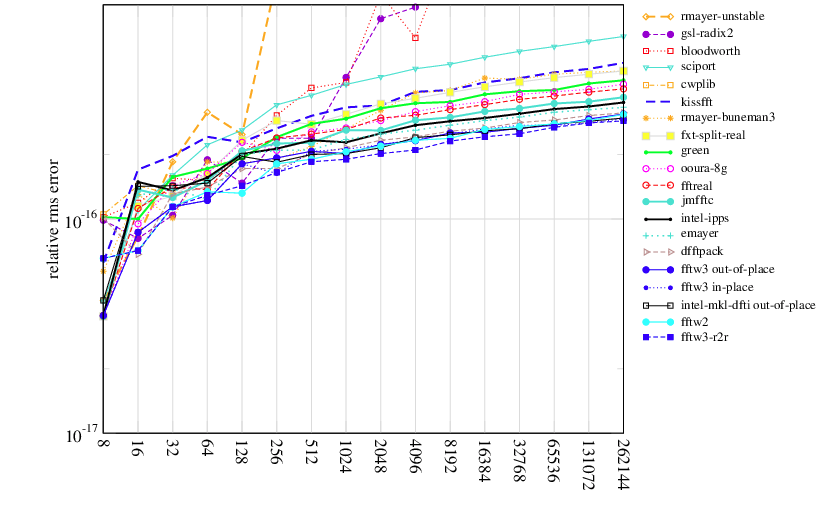
\includegraphics[scale=0.45]{figures/doublefftw.png}
\caption{Double Precision Real data,1 D transforms (Source [\ref{accuracy fftw3}])}
\label{fig:doublea}
\end{figure}
Similarly the relative RMS error in computation of 1D transform of single precision real data is close to a power of $10^{-7}$ for a 2048 point FFT, which is approximately $10^{8}$ times to the error in double precision floating point. 

\begin{figure}[!h]
\centering
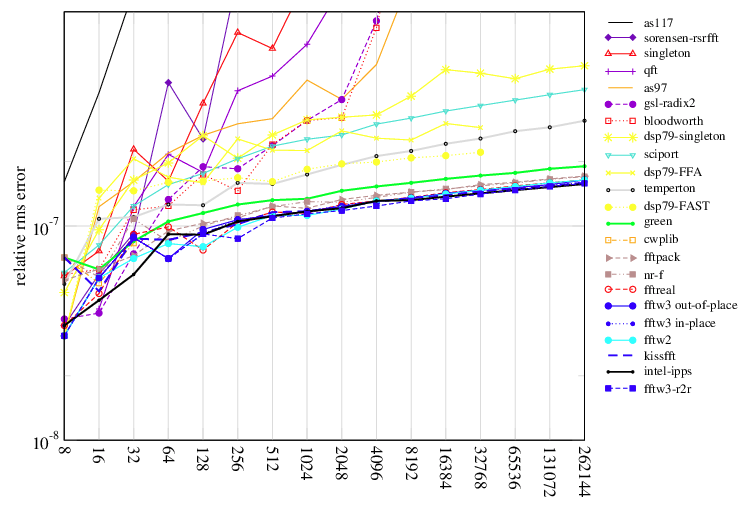
\includegraphics[scale=0.45]{figures/singlefftw.png}
\caption{Single Precision Real data,1 D transforms (Source [\ref{accuracy fftw3}])}
\label{fig:singlea}
\end{figure}
As referenced in the paper [\ref{fhew1}], the error at double precision is in the range $\epsilon$\textsubscript{0}=$2^{-54}$, which matches $\epsilon$\textsubscript{0}.
\begin{math}
\sqrt{log N}
\end{math}, i.e. it grows as the average error for FFT computation O(
\begin{math}
\sqrt{log N}
\end{math}
). The perfect correctness of the computation should be maintained for FFT although rounding the result to floating point doesn't affect the result of NAND computation.
\item
\textbf{Complex Multiplications:}
As part of the \textit{FHEWencrypt}, a number of complex multiplications are computed which aggravate the error.

The code in listing \ref{listing:3.1} demonstrates the complex multiplication step in \textit{FHEWencrypt} function.


\lstset { %
	language=C,
	backgroundcolor=\color{lightgray}, % set backgroundcolor
	%basicstyle=\footnotesize,% basic font setting
	basicstyle=\ttfamily\scriptsize,
	%\basicstyle=\ttfamily\scriptsize,
	keywordstyle=\color{blue}\ttfamily,
	stringstyle=\color{red}\ttfamily,
	commentstyle=\color{darkgray}\ttfamily,
	breaklines=true	
}
\lstset{framesep=-10pt, xleftmargin=-10pt}
\begin{lstlisting}[caption={FHEW:Complex Multiplication Sample},label{listing:1}]
FFTforward(ai, res[i][0]);
     for (int k = 0; k < N2; ++k) 
        ai[k] = ((float complex) ai[k]) * ((float complex) sk_FFT[k]);
        FFTbackward(res[i][1], ai);
\end{lstlisting}



\vspace{0.5cm}
 \noindent The input and output values for the complex multiplication were obtained and thoroughly studied, to deduce the cause of the above output. 
\noindent Table \ref{Table 3.2} provides the results for a single iteration of the above mentioned code to compute complex multiplication.

\vspace{0.25cm}
\begin{table}[!h]
\centering
\caption{FFT Data Comparison For Single Precision and Double Precision for Sample Computation}
\label{Table 3.2}
\begin{tabular}{||m{3cm}|m{1.8cm}|m{4.3cm}|m{4.3cm}||}
\hline
Metric & Variable & Real Part &Imaginary Part\\[1.5ex]
\hline
\hline
\multirow{5}{*}{\parbox{3cm}{Double Precision Floating Point}} & \multicolumn{3}{|c||}{Before Multiplication}\\[1.5ex]\cline{2-4}
  & ai[0] & 17330255872.0000000 &  -706887090176.0000000  \\[1.5ex]\cline{2-4}
&sk\_FFT[0] & 5.646639 &2.667416 \\[1.5ex]\cline{2-4}
& \multicolumn{3}{|c||}{After Multiplication}\\[1.5ex]\cline{2-4}
&ai[0] & 1983419383808.000000 &-3945309667328.000000 \\[1.5ex]
\hline
\hline
\multirow{5}{*}{\parbox{3cm}{Single Precision Floating Point}} & \multicolumn{3}{|c||}{Before Multiplication}\\[1.5ex]\cline{2-4}
&aif[0] & 17330255824.0000000 & -706887090176.0000000   \\[1.5ex]\cline{2-4}
&sk\_FFTF[0] & 5.646641 &2.667419 \\[1.5ex]\cline{2-4}
& \multicolumn{3}{|c||}{After Multiplication}\\[1.5ex]\cline{2-4}
&aif[0] & 1983422005248.000000 &-3945310453760.000000 \\[1.5ex]
\hline
\hline
\multirow{5}{*}{\parbox{3cm}{Difference in Values(double-Single)}} & \multicolumn{3}{|c||}{Before Multiplication}\\[1.5ex]\cline{2-4}
&diff\_ai[0] & 2048.0000000 & 0.0000000   \\[1.5ex]\cline{2-4}
&diff\_sk[0] & -0.000002 &-0.000003 \\[1.5ex]\cline{2-4}
& \multicolumn{3}{|c||}{After Multiplication}\\[1.5ex]\cline{2-4}
&diff\_ai[0] & -2621440.000000 &786432.000000 \\[1.5ex]
\hline
\end{tabular}
\end{table}


\noindent As can be seen from the table \ref{Table 3.2} the difference in the computed values of the variables in double precision and single precision after complex multiplication is significantly large as compared to the difference between the values before the complex multiplication.

\noindent Hence even if the error in values is at $6^{th}$ decimal point for FFT computation it grows upto a large value because of the complex multiplication. Since there are a lot of forward and inverse FFT's happening before the final result of complex multiplication, the algorithm loses accuracy. 
\item
\textbf{Resource Requirements of the Library:} As part of HOMNAND computation, the library computes products of 32 bit integer with 10 bit modulus Q, so a minimum of 42 bits or more are required to store the result.
\end{itemize}

It should be noted that the errors due to floating point approximations doesn't affect the accuracy or functionality of the algorithm, i.e. if the code is modified such that the FFT is computed in double precision and results are rounded off to single precision float, the logical NAND is computed correctly.

\vspace{0.25cm}
\noindent From the above analysis it can be seen that, the algorithm cannot be modified to be implemented in single precision float. Hence accelerator specific modification based on changing the arithmetic cannot be applied to this algorithm because here the modification is at the expense of correctness of the scheme. So further processing of the library is analyzed with double precision FFT. In the following chapter, an analysis is performed to yield a resource optimized implementation of double precision 1024-point FFT for efficient implementation of FHEW on hardware.



